
\section{Mock Samples}
\label{dga:sec:mocks}

Using our parametrization of one-zone GCE models described
in~\S~\ref{dga:sec:onezone}, here we define a set of parameter choices from which
mock samples of stars can be drawn.
We then demonstrate the validity of our likelihood function (Eq.
\ref{dga:eq:likelihood}) in~\S~\ref{dga:sec:mocks:recovered} by applying it to a
fiducial mock sample and comparing the best-fit values to the known parameters
of the input model.
In~\S~\ref{dga:sec:mocks:variations}, we then explore variations in sample size,
measurement precision, and the availability of age information.

\subsection{A Fiducial Mock Sample}
\label{dga:sec:mocks:fiducial}

We take an exponential infall history~$\dot{M}_\text{in} \propto e^{-t /
\tau_\text{in}}$ with an e-folding timescale of~$\tau_\text{in} = 2$ Gyr and an
initial ISM mass of~$M_\text{g} = 0$.
We select an SFE timescale of~$\tau_\star = 15$ Gyr, motivated by the
observational result that dwarf galaxies have generally inefficient star
formation (e.g.,~\citealp{Hudson2015}; though not necessarily halo dwarfs that
formed in denser environments -- see discussion in~\citealt{Naidu2022}).
We additionally select a mass-loading factor of~$\eta = 10$ because the
strength of outflows should, in principle, contain information on the depth of
the gravity well of a given galaxy, with lower mass systems being more
efficient at ejecting material from the ISM.
If the SFH in this model were constant, the analytic formulae of
\citet{Weinberg2017b} suggest that the equilibrium alpha element abundance
should be~$\sim16$\% of the solar oxygen abundance, in qualitative agreement
with the empirical mass-metallicity relation for galaxies
(\citealp{Tremonti2004, Gallazzi2005};~\citealp*{Zahid2011};
\citealp{Andrews2013, Kirby2013, Zahid2014}).
\par
With these choices regarding~$\tau_\star$ and~$\eta$, our parameters are in
the regime where the normalization of the infall history, and consequently the
SFH, is inconsequential to the predicted evolution of the abundances.
The appropriate likelihood function is therefore equation~\refp{dga:eq:likelihood}
with normalized weights, whereas equation~\refp{dga:eq:lnL_minus_weights} with
un-normalized weights would be the proper form if we had selected a
parametrization in which the absolute scale of the SFH impacts the enrichment
history.
Inspection of the average SFHs predicted by the~\textsc{UniverseMachine}
semi-analytic model for galaxy formation~\citep{Behroozi2019} suggests that the
onset of star formation tends to occur a little over~$\sim$13 Gyr ago across
many orders of magnitude in stellar mass extending as low as
$\text{M}_\star \approx 10^{7.2}~\msun$.
We therefore assume that the onset of star formation occurred~$\sim$13.2 Gyr
ago, allowing~$\sim$500 Myr between the Big Bang and the first stars.
We evolve this model for 10 Gyr exactly (i.e., the youngest stars in the mock
sample have an exact age of 3.2 Gyr), stopping short of 13.2 Gyr because
surviving dwarf galaxies and stellar streams often have their star formation
quenched (e.g.,~\citealp{Monelli2010a, Monelli2010b, Sohn2013, Weisz2014a,
Weisz2014b, Weisz2015}).
These choices are not intended to resemble any one galaxy, but instead to
qualitatively resemble some disrupted dwarf galaxy whose evolutionary
parameters can be re-derived using our likelihood function as a check that it
produces accurate best-fit parameters.
\par
As discussed in~\S~\ref{dga:sec:onezone}, thoughout this paper we assume that the
IMF-averaged alpha element yield is exactly~$\yacc = 0.01$ and
$y_\alpha^\text{Ia} = 0$.
While loosely motivated by nucleosynthesis models in massive stars
\citep[e.g.,][]{Nomoto2013, Sukhbold2016, Limongi2018}, this choice is intended
to set some normalization of the effective yields which can be scaled up or
down to accommodate alternative choices.
If no scale is assumed, then extremely strong degeneracies arise in the
inferred yields, the strength of outflows~$\eta$, and the SFE timescale
$\tau_\star$ due to the yield-outflow degeneracy (see discussion in
Appendix~\ref{dga:sec:degeneracy}).
We do not distinguish between alpha elements in this validation of our
likelihood function because, from a modelling standpoint, they can all be
treated the same with a metallicity-independent yield from CCSNe and negligible
yields from all other sources (at least for the lighter alpha elements such as
O and Mg;~\citealp{Johnson2019}).
In practice, however, we take O as the canonical alpha element when integrating
these models with~\vice, adopting~$Z_{\text{O},\odot} = 0.00572$ as the
abundance of O in the sun according to~\citet{Asplund2009} and consistent with
the recent revisions of~\citet*{Asplund2021}, though similar~\afe~ratios would
arise anyway if we instead took, e.g., Mg and asserted that [O/Mg]~$\approx 0$.
\par
\citet{Weinberg2017b} adopt~$\yacc = 0.015$,~$\yfecc = 0.0012$ and
$\yfeia = 0.0017$ (see discussion in their~\S~2.2).
This massive star yield of Fe is appropriate for nucleosynthesis models in
which most~$M > 8~\msun$ stars explode as a CCSN~\citep[e.g.,][]{Woosley1995,
Chieffi2004, Chieffi2013, Nomoto2013} assuming a~\citet{Kroupa2001} IMF.
This SN Ia yield of Fe is based on the W70 explosion model of
\citet{Iwamoto1999} which produces~$\sim$0.77~\msun~of Fe per SN Ia event and
assuming that~$\scinote{2.2}{-3}~\msun^{-1}$ SNe Ia arise per solar mass of
star formation based on~\citet{Maoz2012a}.
Following these arguments, we scale these yields down by factors of~$\sim$2/3
such that $\yacc = 0.01$, adopting~$\yfecc = \scinote{8}{-4}$ and
$\yfeia = \scinote{1.1}{-3}$ in our mock samples.
We retain the assumption that~$\yacc = 0.01$ in our fits to our mock samples
but otherwise let the Fe yields~\yfecc~and~\yfeia~be free parameters to be
recovered by our likelihood function.
We use this procedure in our application to the H3 survey in~\S~\ref{dga:sec:h3}
below as well.
We then sample~$N = 500$ stars from the underlying SFH each of which have -- in
the interest of mimicking the typical precision achieved by a spectroscopic
survey of a local group dwarf galaxy --~$\sigma_\afe = \sigma_\feh = 0.05$.
100 of these stars have age measurements with an uncertainty of
$\sigma_{\log_{10}(\text{age})} = 0.1$ (i.e.,~$\sim$23\% precision).

\subsection{Recovered Parameters of the Fiducial Mock}
\label{dga:sec:mocks:recovered}

% fig 2
\begin{figure*}
\centering
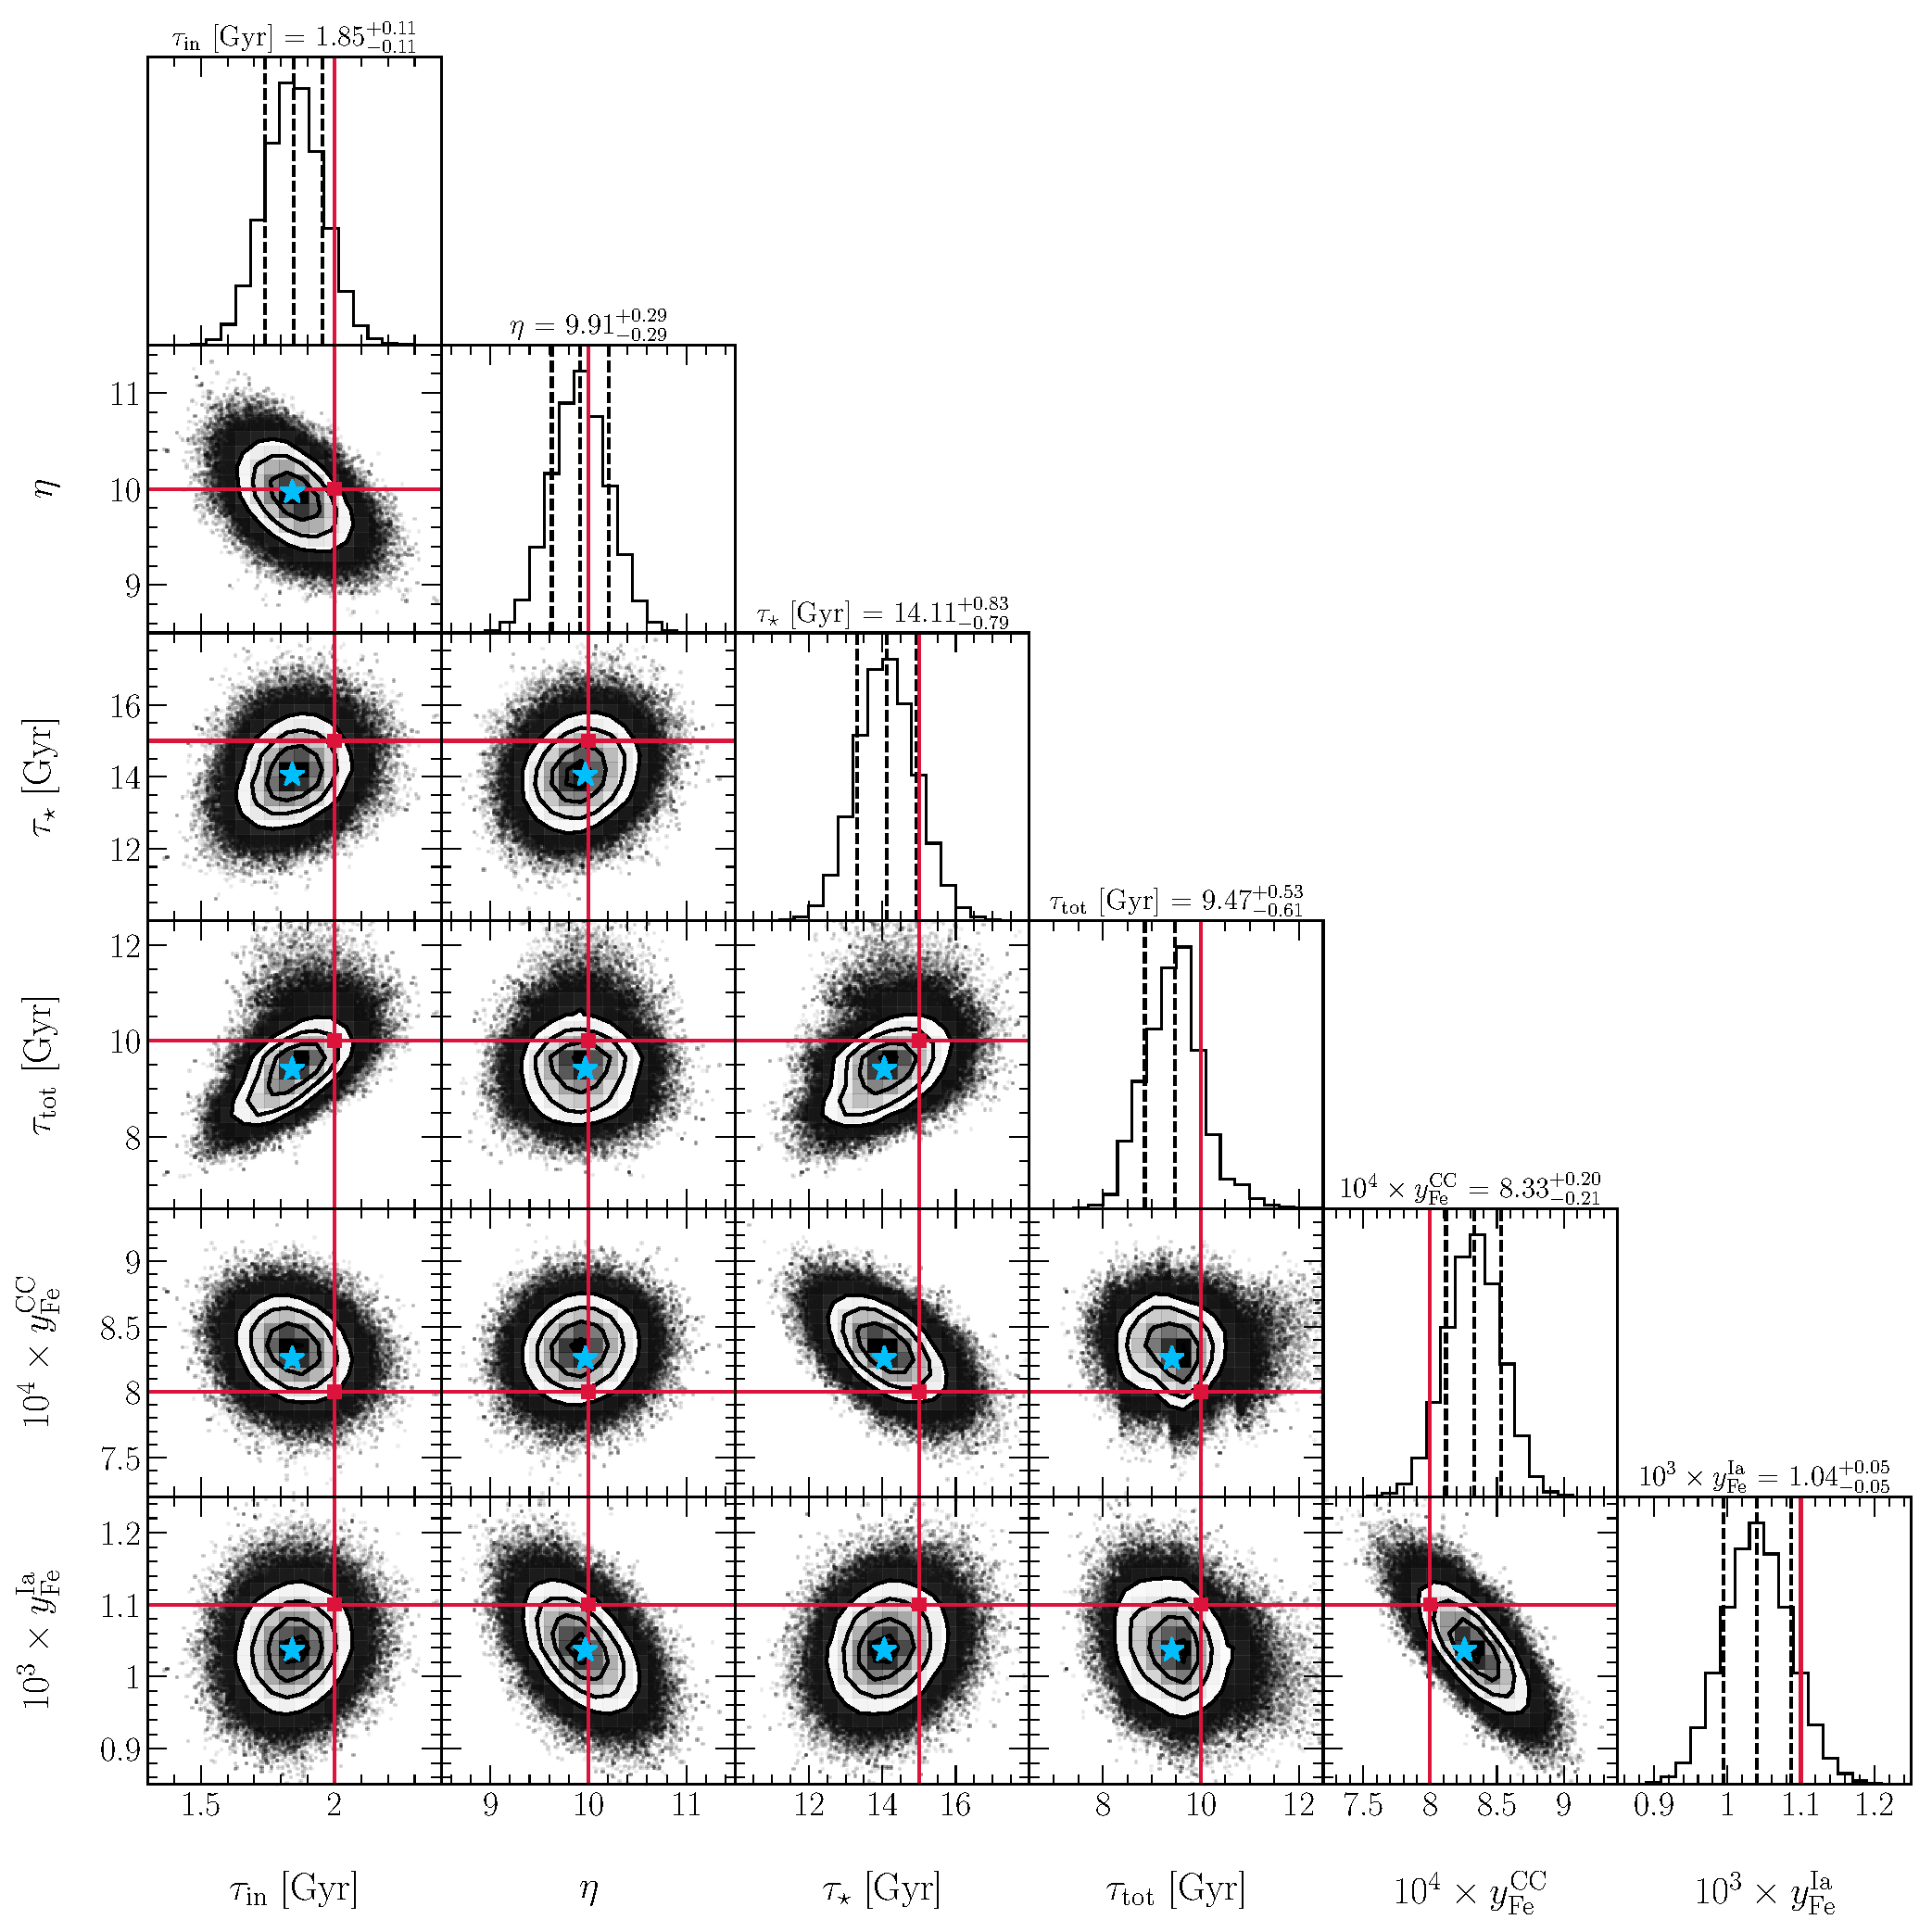
\includegraphics[scale = 0.42]{fiducial_512k.pdf}
\caption{
Posterior distributions obtained from applying our fitting method to our
fiducial mock sample (see Fig.~\ref{dga:fig:fiducial_mock} and discussion
in~\S\S~\ref{dga:sec:fitting} and~\ref{dga:sec:mocks:fiducial}).
Panels below the diagonal show 2-dimensional cross-sections of the likelihood
function while panels along the diagonal show the marginalized distributions
along with the best-fit values and confidence intervals.
Blue stars mark the element of the Markov chain with the maximum likelihood.
Red ``cross-hairs'' denote the true, known values of the parameters from the
input model (see the top row of Table~\ref{dga:tab:recovered_values}).
}
\label{dga:fig:fiducial_mock_corner}
\end{figure*}

Fig.~\ref{dga:fig:fiducial_mock} shows our fiducial mock in the observed space.
As intended by our parameter choices (see discussion
in~\S~\ref{dga:sec:mocks:fiducial}), this sample qualitatively resembles a typical
disrupted dwarf galaxy -- dominated by old stars with metal-poor
($\feh \approx -1$) and alpha-enhanced ($\afe \approx +0.2$) modes in the MDF.
We now apply the method outline in~\S~\ref{dga:sec:fitting} to recover the known
parameters of the input model.
Fig.~\ref{dga:fig:fiducial_mock_corner} shows the resulting posterior distributions,
demonstrating that our likelihood function accurately recovers each parameter.
We include the predictions of the best-fit model in Fig.~\ref{dga:fig:fiducial_mock},
finding excellent agreement with the input model.
To quantify the quality of the fit, for each datum~$\script{D}_i$ we find the
point along the track~$\script{M}_j$ with the maximum likelihood of observation
(i.e.,~$\{\script{D}_i,\script{M}_j~|~\ln L(\script{D}_i | \script{M}_j) =
\max(\ln L(\script{D}_i | \script{M}))\}$).
We then compute the chi-squared per degree of freedom diagnostic according to
\begin{equation}
\chi_\text{dof}^2 = \frac{1}{N_\text{obs} - N_\theta}
\sum_{i,j} \Delta_{ij} C_i^{-1} \Delta_{ij}^T,
\label{dga:eq:chisquared_dof}
\end{equation}
where~$N_\text{obs}$ is the number of quantities in the observed sample,
$N_\theta$ is the number of model parameteres, and the summation is taken over
the pair-wise combinations of the data and model with the maximum likelihood of
observation.
Although marginalizing over the track~\script{M}~is necessary to derive
accurate best-fit parameters (see discussion below and in~\S~\ref{dga:sec:fitting}),
it should be safe to estimate the quality of a fit by simply pairing each datum
with the most appropriate point on the track.
As noted in the middle panel of Fig.~\ref{dga:fig:fiducial_mock}, our method
achieves~$\chi_\text{dof}^2 = 0.55$, indicating that we have perhaps
over-parametrized the data.
This result is unsurprising, however, because we have fit the mock data with
the exact, known parametrization of the evolutionary history and
nucleosynthetic yields of the input model in the interest of demonstrating
proof of concept that equation~\refp{dga:eq:likelihood} provides accurate best-fit
values.
\par
Although it may appear that there are a worrying number of~$\gtrsim 1\sigma$
discrepancies in Fig.~\ref{dga:fig:fiducial_mock_corner}, we demonstrate
in~\S~\ref{dga:sec:mocks:variations} below that the differences between the known
and best-fit values here are consistent with randomly sampling from a Gaussian
distribution due to measurement uncertainty.
Although most cross sections of the posterior distribution are sufficiently
described by a multivariate Gaussian, there is some subtructure in the
likelihood distribution of~$\tau_\text{in}$, most noticeable in the
$\yfecc - \tau_\text{in}$ plane.
The MCMC algorithm naturally catches this structure, but it would be missed
under the assumption of Gaussianity as in, e.g., maximum a posteriori estimates.
There are a handful of degeneracies in the likelihood distribution of the
recovered parameters, which arise as a consequence of having an impact on the
same observable.
We discuss them individually below.
\par
% \textit{The centroid of the MDF.}
% With a fixed alpha element yield of~$\yacc = 0.01$ as we have adopted here,
% the strength of outflows~$\eta$ is set by ensuring the centroid of
% the~\ah~distribution is in agreement with the data.
% This in turn requires a total Fe yields of~$\yfecc + \yfeia$ which corresponds
% to the centroid of the~\feh~distribution.
% The total Fe yield, however, can be achieved with different breakdowns between
% CCSN and SN Ia enrichment, giving rise to the inverse relationship
% between the two Fe yields.
% \par
\textit{The height of the ``plateau'' and position of the ``knee'' in the
evolutionary track.}
The plateau in the~\afe-\feh~plane occurs in our input model
at~$\afe_\text{CC} \approx +0.45$ and arises due to the IMF-averaged massive
star yields of alpha and iron-peak elements.
The knee occurs thereafter with the onset of SN Ia enrichment, a
nucleosynthetic source of Fe but negligible amounts of alpha elements like O
and Mg~\citep{Johnson2019}.
With fixed~\yacc, variations in~\yfecc~adjust the vertical height of the
plateau.
\citet{Weinberg2017b} demonstrate that, to first order, the SFE timescale
$\tau_\star$ determines the metallicity~\feh~at which the knee occurs with
low~$\tau_\star$ models predicting a knee at high~\feh.
If a lowered plateau (i.e., higher~\yfecc) is accompanied by faster star
formation (i.e., lower~$\tau_\star$), the portion of the evolutionary track
in which~\afe~is decreasing occurs in a similar region of chemical space.
\yfecc~and~$\tau_\star$ are therefore inversely related when an overall scale
of nucleosynthetic yields is chosen.
When the overall scale is allowed to vary, we find a degeneracy of the opposite
sign (see discussion in Appendix~\ref{dga:sec:degeneracy}).
\par
\textit{The endpoint of the model track and centroid of the MDF.}
% The ratio~$\yfecc / \yfeia$ controls the drop in~\afe~between the plateau
% and the equilibrium~\afe.
These are the regions of chemical space where most of the
data are generally found, so for a given choice of~$\eta$, the~\textit{total}
Fe yield is well constrained observationally.
With only the total precisely determined,~\yfecc~and~\yfeia~are inversely
related.
On its own, adjusting~\yfeia~shifts the track vertically in the~\afe-\feh~plane
(there is horizontal movement as well, though the vertical movement is
stronger).
A downward shift in the predicted track (i.e., and increase in~$\yfeia$) can be
accompanied by a rightward shift (i.e., a decrease in~$\eta$) such that the
endpoint lies in the same location as the data.
$\yfeia$ and~$\eta$ are therefore inversely related, whereas the yield-outflow
degeneracy produces a direct relationship between these parameters
(see Appendix~\ref{dga:sec:degeneracy}).
\par
\textit{The shape of the MDF.}
The~\afe~and~\feh~distributions are affected in a handful of ways by the
parameters of this input model.
The duration of star formation has the simplest effect of cutting off the MDF
at some abundance.
Inefficient star formation (i.e., high~$\tau_\star$) increases the frequency of
low metallicity stars because it takes significantly longer for the ISM to
reach the equilibrium abundance.
Sharp infall histories (i.e., low~$\tau_\text{in}$) predict wide MDFs because
the ISM mass declines with time through losses to star formation and the lack
of replenishment by accretion.
Metals are then deposited into a ``gas-starved'' reservoir, which then reaches
higher abundances due to a deficit of hydrogen and helium.
This effect is particularly strong for Fe because of the delayed nature of SN
Ia enrichment~\citep{Weinberg2017b}.
These models achieve higher metallicities in the ISM, but their declining SFHs
produce a larger fraction of their stars early in their evolutionary history
when the abundances are lower than the late-time equilibrium abundance.
Consequently, the MDF that arises is wider for sharp infall histories but has
a peak in a similar position regardless of~$\tau_\text{in}$.
Folding these effects together, degeneracies arise in the inferred parameters
as a consequence of their effects on the MDF.
Between~$\tau_\text{in}$ and~$\tau_\text{tot}$, a sharp infall history can
broaden the MDF, but cutting off star formation earlier can allow the
distribution to remain peaked if the data suggest it.
Similarly, efficient star formation (i.e., low~$\tau_\star$) allows the ISM to
spend more time near its equilibrium abundance, enhancing the peak of the MDF,
but this change in shape can be reversed by cutting off star formation.
Between~$\tau_\text{in}$ and~$\eta$, a sharp infall history gives rise to a
high metallicity tail of the MDF, but increasing the strength of outflows
can lower the overall metallicity if this tail is too metal-rich compared to
the data.
\par
We emphasize that our fits achieve this level of precision by selecting an
overall scale for nucleosynthetic yields and outflows ($\yacc = 0.01$; see
discussion in~\S~\ref{dga:sec:onezone} and Appendix~\ref{dga:sec:degeneracy}).
Any GCE parameter that influences the centroid of the MDF or the position or
shape of the evolutionary track in abundance space is subject to the
yield-outflow degeneracy.
Given an overall scale of yields, set here by choosing~\yacc, a sample like
our fiducial mock gives quite precise constraints on all model parameters.
If we modify our choice of~\yacc, we would find similar predictions by
adjusting our Fe yields,~$\tau_\star$ and~$\eta$.
If~\yacc~is instead allowed to vary as a free parameter, then the degeneracies
are strong, but~$\tau_\text{in}$ and~$\tau_\text{tot}$ remain well constrained
due to their impact on the MDF shape.
% This includes all evolutionary parameters in our input model with the exception
% of~$\tau_\text{in}$ and~$\tau_\text{tot}$ because they impact only the shape of
% the MDF, an observational diagnostic which is constrained by a sufficiently
% large sample.
% We discuss the implications of these results applied to observed data
% in~\S~\ref{dga:sec:mocks:variations} below.
\par
In conducting these tests against mock samples, we find that the two central
features of this method are essential to ensuring the accuracy of the best-fit
parameters.
When either the weighted likelihood or the marginalization over the track
(see discussion in~\S~\ref{dga:sec:fitting}) are omitted, the fit fails to recover
the parameters of the input model with discrepancies at the many-$\sigma$ level
between the best-fit and known values.
For this reason, we caution against the reliability of GCE parameters inferred
from simplified likelihood estimates, such as matching each datum with the
nearest point on the track.


\afterpage{
\captionsetup{width=\textheight}
\begin{singlespace}
\clearpage
\renewcommand{\arraystretch}{1.5}
\begin{landscape}
% \begin{table*}
\begin{longtable}{l @{\extracolsep{\fill}} c c c c c c}
\caption{
Known (top row) and recovered best-fit values of the evolutionary parameters
of the input GCE model to out mock samples.
From left to right: the variation of our fiducial mock sample, the e-folding
timescale of the infall history~$\tau_\text{in}$, the outflow mass-loading
factor~$\eta$, the SFE timescale~$\tau_\star$, the duration of star formation
$\tau_\text{tot}$, the IMF-averaged Fe yield from CCSNe~\yfecc~and the
DTD-integrated Fe yield from SNe Ia~\yfeia.
Each variation has the same evolutionary parameters as the input model, but
has either a different sample size (top block), measurement uncertainty
in~\feh~and~\afe~abundances (top-middle block), measurement uncertainty
in~$\log_{10}(\text{age})$ (bottom-middle block), or fraction of the
sample with available age measurements (bottom block).
The values taken in the fiducial mock sample are marked in bold.
We provide illustrations of the accuracy and precision of these fits in
Figs.~\ref{dga:fig:accuracy} and~\ref{dga:fig:precision}, respectively.
}
\\
% \begin{tabularx}{\linewidth}{l @{\extracolsep{\fill}} c c c c c c}
\hline
Mock Sample & $\tau_\text{in}$ [Gyr] & $\eta$ & $\tau_\star$ [Gyr] &
$\tau_\text{tot}$ [Gyr] & \yfecc~[$\times 10^{-4}$] & \yfeia~[$\times 10^{-3}$]
\\
\hline
\null &
2 &
10  &
15 &
10 &
8.00 &
1.10
\\
\hline
$N = 20$ &
$2.55^{+0.75}_{-0.45}$ &
$8.39^{+1.11}_{-1.30}$  &
$14.35^{+5.56}_{-3.32}$ &
$10.60^{+1.65}_{-1.09}$ &
${7.90^{+1.20}_{-1.90}}$ &
${1.36^{+0.33}_{-0.23}}$
\\
$N = 50$ &
$2.13^{+0.42}_{-0.36}$ &
$10.39^{+0.80}_{-0.76}$  &
$13.75^{+2.79}_{-2.38}$ &
$11.25^{+1.37}_{-1.76}$ &
${8.30 \pm 0.60}$ &
${0.95 \pm 0.14}$
\\
$N = 100$ &
$2.06^{+0.27}_{-0.26}$ &
$9.88^{+0.64}_{-0.62}$  &
$15.06^{+2.00}_{-1.79}$ &
$11.52^{+1.06}_{-1.30}$ &
$8.10 \pm 0.40$ &
$1.08 \pm 0.09$
\\
$N = 200$ &
$2.10^{+0.18}_{-0.17}$ &
$10.11^{+0.45}_{-0.43}$  &
$14.61^{+1.34}_{-1.18}$ &
$10.60^{+1.07}_{-0.86}$ &
$7.70 \pm 0.30$ &
$1.14 \pm 0.07$
\\
$\bm{N = 500}$ &
$\bm{1.85 \pm 0.11}$ &
$\bm{9.91 \pm 0.29}$  &
$\bm{14.11^{+0.83}_{-0.79}}$ &
$\bm{9.47^{+0.53}_{-0.61}}$ &
$\bm{8.30^{+0.20}_{-0.21}}$ &
$\bm{1.04 \pm 0.05}$
\\
$N = 1000$ &
$2.05^{+0.09}_{-0.08}$ &
$9.72 \pm 0.20$  &
$14.62^{+0.57}_{-0.56}$ &
$9.83^{+0.38}_{-0.39}$ &
$8.10 \pm 0.10$ &
$1.14 \pm 0.03$
\\
$N = 2000$ &
$2.00 \pm 0.05$ &
$10.26 \pm 0.15$  &
$15.82^{+0.44}_{-0.42}$ &
$10.30^{+0.25}_{-0.32}$ &
$8.00 \pm 0.10$ &
$1.09 \pm 0.02$
\\
\hline
$\sigma_\text{[X/Y]} = 0.01$ &
$1.89 \pm 0.10$ &
$10.25 \pm 0.28$  &
$15.06^{+0.52}_{-0.47}$ &
$9.70^{+0.51}_{-0.59}$ &
$8.00 \pm 0.10$ &
$1.09 \pm 0.02$
\\
$\sigma_\text{[X/Y]} = 0.02$ &
$1.92^{+0.10}_{-0.09}$ &
$10.10 \pm 0.25$  &
$14.71^{+0.56}_{-0.55}$ &
$9.79^{+0.45}_{-0.40}$ &
$8.10 \pm 0.10$ &
$1.08^{+0.02}_{-0.03}$
\\
$\bm{\sigma_\textbf{[X/Y]} = 0.05}$ &
$\bm{1.85 \pm 0.11}$ &
$\bm{9.91 \pm 0.29}$  &
$\bm{14.11^{+0.83}_{-0.79}}$ &
$\bm{9.47^{+0.53}_{-0.61}}$ &
$\bm{8.30^{+0.20}_{-0.21}}$ &
$\bm{1.04 \pm 0.05}$
\\
$\sigma_\text{[X/Y]} = 0.1$ &
$2.00^{+0.13}_{-0.12}$ &
$9.88^{+0.31}_{-0.33}$  &
$13.39 \pm 1.02$ &
$11.10^{+1.00}_{-0.84}$ &
$8.50^{+0.40}_{-0.30}$ &
$1.01 \pm 0.07$
\\
$\sigma_\text{[X/Y]} = 0.2$ &
$2.22 \pm 0.21$ &
$9.83^{+0.58}_{-0.67}$  &
$18.21^{+2.19}_{-2.02}$ &
$10.32^{+1.05}_{-0.67}$ &
$8.70 \pm 0.70$ &
$1.05 \pm 0.14$
\\
$\sigma_\text{[X/Y]} = 0.5$ &
$2.73^{+0.82}_{-0.60}$ &
$10.05^{+1.22}_{-1.26}$  &
$12.52^{+3.75}_{-3.35}$ &
$9.00^{+1.26}_{-0.95}$ &
$7.50^{+1.80}_{-1.60}$ &
$1.12 \pm 0.31$
\\
\hline
$\sigma_{\log_{10}(\text{age})} = 0.02$ &
$2.08^{+0.09}_{-0.08}$ &
$9.84^{+0.24}_{-0.26}$  &
$14.69^{+0.50}_{-0.46}$ &
$10.41^{+0.47}_{-0.41}$ &
$8.10 \pm 0.20$ &
$1.11^{+0.05}_{-0.04}$
\\
$\sigma_{\log_{10}(\text{age})} = 0.05$ &
$1.96 \pm 0.11$ &
$9.88^{+0.32}_{-0.30}$  &
$15.70^{+0.71}_{-0.68}$ &
$9.95^{+0.63}_{-0.53}$ &
$8.00 \pm 0.20$ &
$1.11^{+0.05}_{-0.04}$
\\
$\bm{\sigma_{\log_{10}(\textbf{age})} = 0.1}$ &
$\bm{1.85 \pm 0.11}$ &
$\bm{9.91 \pm 0.29}$  &
$\bm{14.11^{+0.83}_{-0.79}}$ &
$\bm{9.47^{+0.53}_{-0.61}}$ &
$\bm{8.30^{+0.20}_{-0.21}}$ &
$\bm{1.04 \pm 0.05}$
\\
$\sigma_{\log_{10}(\text{age})} = 0.2$ &
$2.20^{+0.18}_{-0.17}$ &
$9.83^{+0.28}_{-0.27}$  &
$15.19 \pm 1.11$ &
$10.76^{+0.85}_{-0.93}$ &
$8.00 \pm 0.20$ &
$1.11^{+0.05}_{-0.04}$
\\
$\sigma_{\log_{10}(\text{age})} = 0.5$ &
$2.25^{+0.20}_{-0.25}$ &
$9.86^{+0.28}_{-0.30}$  &
$16.24^{+1.44}_{-1.62}$ &
$11.38^{+1.00}_{-1.34}$ &
$8.00 \pm 0.20$ &
$1.10 \pm 0.05$
\\
$\sigma_{\log_{10}(\text{age})} = 1$ &
$1.69^{+0.35}_{-0.32}$ &
$9.53 \pm 0.29$  &
$12.38^{+2.27}_{-2.08}$ &
$8.66^{+1.86}_{-1.74}$ &
$8.30 \pm 0.30$ &
$1.15 \pm 0.06$
\\
\hline
$f_\text{age} = 0$ &
$1.65^{+0.55}_{-0.37}$ &
$9.39^{+0.30}_{-0.29}$  &
$11.80^{+3.36}_{-2.44}$ &
$7.35^{+2.62}_{-1.74}$ &
$8.30 \pm 0.40$ &
$1.19^{+0.08}_{-0.07}$
\\
$f_\text{age} = 0.1$ &
$1.75^{+0.16}_{-0.17}$ &
$10.06^{+0.29}_{-0.28}$  &
$13.65^{+1.22}_{-1.12}$ &
$8.84 \pm 0.87$ &
$8.40 \pm 0.20$ &
$1.06 \pm 0.05$
\\
$\bm{f_\textbf{age} = 0.2}$ &
$\bm{1.85 \pm 0.11}$ &
$\bm{9.91 \pm 0.29}$  &
$\bm{14.11^{+0.83}_{-0.79}}$ &
$\bm{9.47^{+0.53}_{-0.61}}$ &
$\bm{8.30^{+0.20}_{-0.21}}$ &
$\bm{1.04 \pm 0.05}$
\\
$f_\text{age} = 0.3$ &
$1.94^{+0.11}_{-0.10}$ &
$9.80^{+0.27}_{-0.28}$  &
$14.26^{+0.74}_{-0.67}$ &
$9.89^{+0.54}_{-0.48}$ &
$8.00 \pm 0.20$ &
$1.10 \pm 0.04$
\\
$f_\text{age} = 0.4$ &
$1.91^{+0.09}_{-0.10}$ &
$10.07^{+0.32}_{-0.30}$  &
$16.79^{+0.81}_{-0.83}$ &
$10.34^{+0.61}_{-0.50}$ &
$7.80 \pm 0.20$ &
$1.12 \pm 0.05$
\\
$f_\text{age} = 0.5$ &
$2.00 \pm 0.10$ &
$10.16^{+0.30}_{-0.29}$  &
$15.46^{+0.70}_{-0.69}$ &
$9.83^{+0.48}_{-0.40}$ &
$7.80 \pm 0.20$ &
$1.12^{+0.05}_{-0.04}$
\\
$f_\text{age} = 0.6$ &
$2.18 \pm 0.09$ &
$9.65^{+0.27}_{-0.25}$  &
$14.25^{+0.67}_{-0.64}$ &
$10.49^{+0.44}_{-0.37}$ &
$7.80 \pm 0.20$ &
$1.15 \pm 0.04$
\\
$f_\text{age} = 0.7$ &
$1.99 \pm 0.08$ &
$9.81^{+0.28}_{-0.27}$  &
$14.92^{+0.68}_{-0.62}$ &
$10.25^{+0.46}_{-0.37}$ &
$8.10 \pm 0.20$ &
$1.08 \pm 0.04$
\\
$f_\text{age} = 0.8$ &
$2.06 \pm 0.09$ &
$9.53^{+0.29}_{-0.26}$  &
$15.18^{+0.63}_{-0.59}$ &
$9.76^{+0.36}_{-0.33}$ &
$7.90 \pm 0.20$ &
$1.15 \pm 0.05$
\\
$f_\text{age} = 0.9$ &
$1.93 \pm 0.08$ &
$10.41 \pm 0.31$  &
$16.23^{+0.73}_{-0.70}$ &
$10.03^{+0.39}_{-0.33}$ &
$7.70 \pm 0.20$ &
$1.14 \pm 0.04$
\\
$f_\text{age} = 1$ &
$2.13 \pm 0.09$ &
$9.44^{+0.28}_{-0.27}$  &
$15.67^{+0.64}_{-0.60}$ &
$10.21^{+0.35}_{-0.31}$ &
$8.00 \pm 0.20$ &
$1.15 \pm 0.05$
\\
\hline
% \end{tabularx}
\label{dga:tab:recovered_values}
% \end{table*}
\end{longtable}
\end{landscape}
\clearpage
\end{singlespace}
} % afterpage



% fig 3
\begin{figure*}
\centering
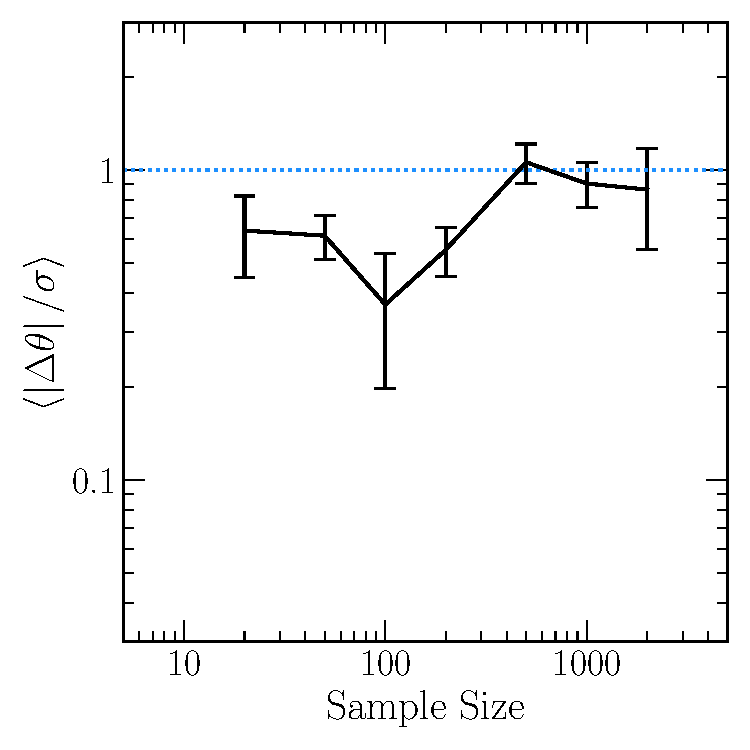
\includegraphics[scale = 0.42]{dp_sigma_samplesize.pdf}
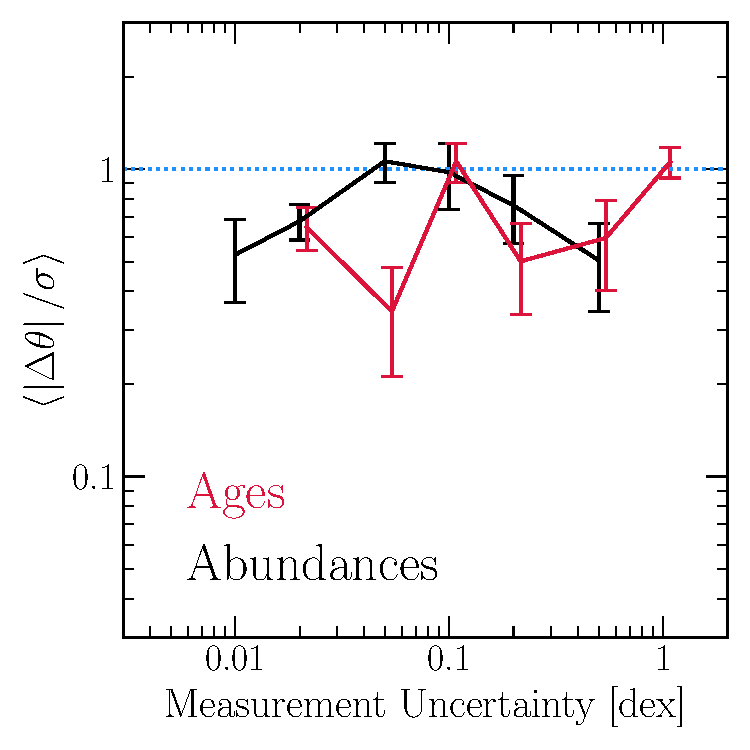
\includegraphics[scale = 0.42]{dp_sigma_precision.pdf}
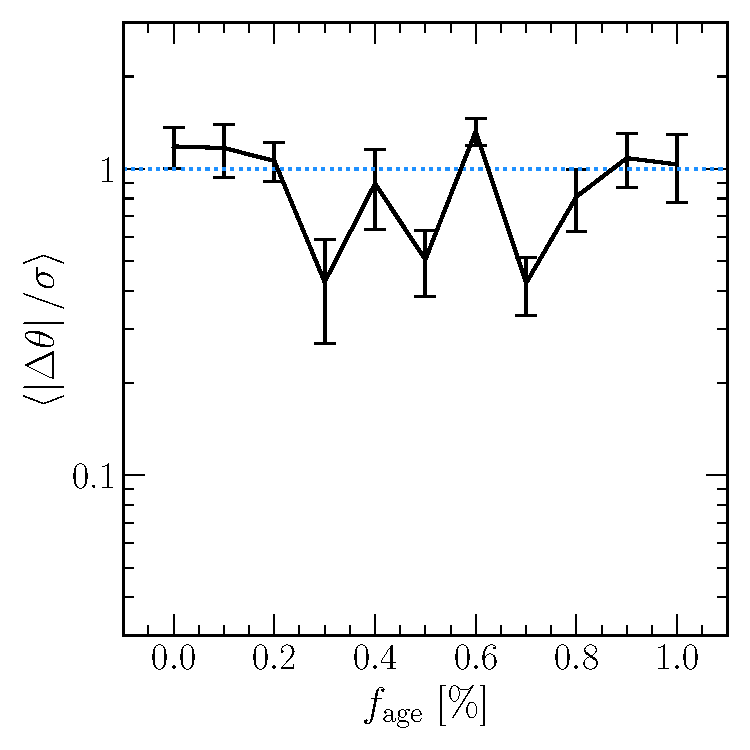
\includegraphics[scale = 0.42]{dp_sigma_agefrac.pdf}
\caption{
Differences between input model parameters and recovered best-fit values.
Each point is the mean deviation~$\left|\Delta\theta\right|$ for each of the
six free parameters in Table~\ref{dga:tab:recovered_values} (i.e.,
$\{\theta\} = \{\tau_\text{in}, \eta, \tau_\star, \tau_\text{tot}, \yfecc,
\yfeia\}$) in units of the best-fit uncertainty~$\sigma$.
Our mock samples vary in terms of their sample size (left), measurement
precision in~\feh~and~\afe~abundances (middle, black), measurement precision in
$\log_{10}(\text{age})$ (middle, red), and the fraction of the sample with
available age measurements (right).
Error bars denote the error in the mean deviation of the six free parameters.
Blue dotted lines mark~$\langle \Delta \theta / \sigma \rangle = 1$, the
expected mean offset due to randomly sampling from a Gaussian distribution.
}
\label{dga:fig:accuracy}
\end{figure*}

\subsection{Variations in Sample Size, Measurement Precision and the
Availability of Age Information}
\label{dga:sec:mocks:variations}

We now explore variations of our fiducial mock sample.
We retain the same evolutionary parameters of the input model (see discussion
in~\S~\ref{dga:sec:mocks:fiducial}), but each variant differs in one of the
following:
\begin{itemize}

	\item Sample size.

	\item Measurement precision in~\feh~and~\afe.

	\item Measurement precision in~$\log_{10}(\text{age})$.

	\item The fraction of the sample that has age measurements.

\end{itemize}
The left-hand column of Table~\ref{dga:tab:recovered_values} provides a summary of
the values we take as exploratory cases with the fiducial mock marked in bold.
In the remaining columns, we provide the associated values derived for each
GCE parameter~$\theta$ along with their~$1\sigma$ confidence intervals.
The sample sizes we consider are intended to reflect the range that is
typically achieved in disrupted dwarf galaxies where the proximity might
allow individual age estimates for main sequence turnoff stars.
Because of their distance and low stellar mass, dwarf galaxies are considerably
less conducive to the large sample sizes achieved by Milky Way surveys like
APOGEE~\citep{Majewski2017} and GALAH~\citep{DeSilva2015, Martell2017}.
Our choices in measurement precision are intended to reflect typical values
achieved by modern spectroscopic surveys.
Although deriving elemental abundances through spectroscopy is a nontrivial
problem known to be affected by systematics~\citep[e.g.,][]{Anguiano2018},
stellar age measurements
are generally the more difficult of the two~\citep{Soderblom2010, Chaplin2013}.
The age measurements may therefore be available for only a small portion of the
sample and are often less precise than the abundances ($f_\text{age} = 20$\%
and~$\sigma_\feh = \sigma_\afe = 0.05$ versus
$\sigma_{\log_{10}(\text{age})} = 0.1$ in our fiducial mock).
In practice, however, uncertainties vary with stellar mass; for example, hot
main sequence turnoff stars have precise ages but poorly constrained
abundances due to the lack of lines in their spectra.
\par
Fig.~\ref{dga:fig:accuracy} demonstrates the accuracy of our fitting method with
respect to variations in these details surrounding the data.
We compute the deviation between each re-derived parameter~$\theta$
(i.e.,~$\tau_\text{in}$,~$\eta$,~$\tau_\star$, etc.) and its known value from
the input model, then divide by the fit uncertainty~$\sigma_\theta$ and plot
the mean on the y-axis.
Under all variants that we explore, our likelihood function accurately recovers
the input parameters to~$\sim1\sigma$ or slightly better.
This deviation is exactly as expected when the uncertainties are described by a
Gaussian random process, wherein the most likely deviation from the true value
is exactly~$1\sigma$.
This expectation holds even with infinite data, though in that limit
the~$1\sigma$ uncertainty interval becomes arbitrarily small.
This demonstrates that equation~\refp{dga:eq:likelihood} provides accurate best-fit
parameters even when the sample size is as low as~$N \approx 20$, when the
measurement uncertainties are as imprecise as~$\sigma_\text{[X/Y]} \approx 0.5$
and~$\sigma_{\log_{10}(\text{age})} \approx 1$, or even when there is no age
information available at all.
The precision of the fit will indeed suffer in such cases (see Fig.
\ref{dga:fig:precision} and associated discussion below), but the inferred
parameters will remain accurate nonetheless.

% fig 4
\begin{figure*}
\centering
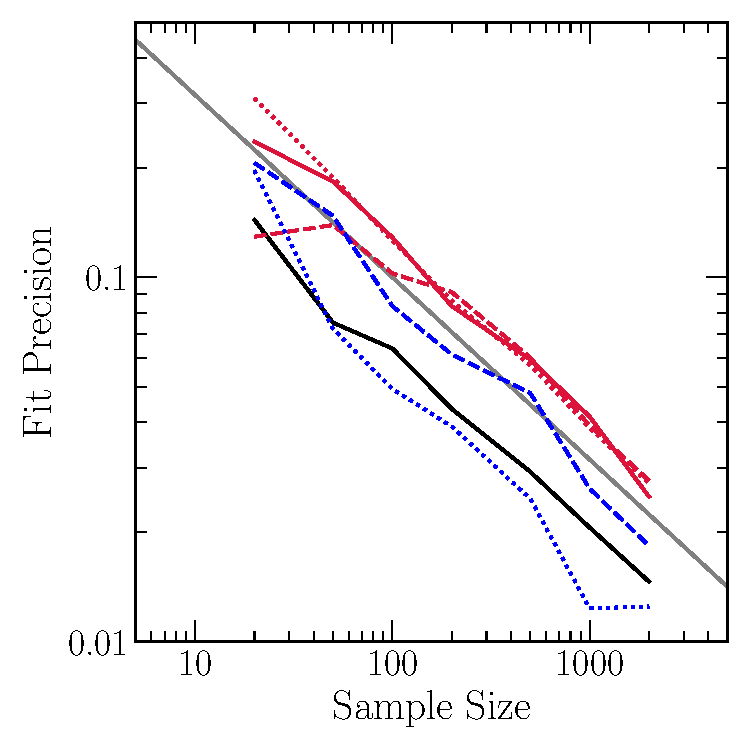
\includegraphics[scale = 0.55]{precision_samplesize.pdf}
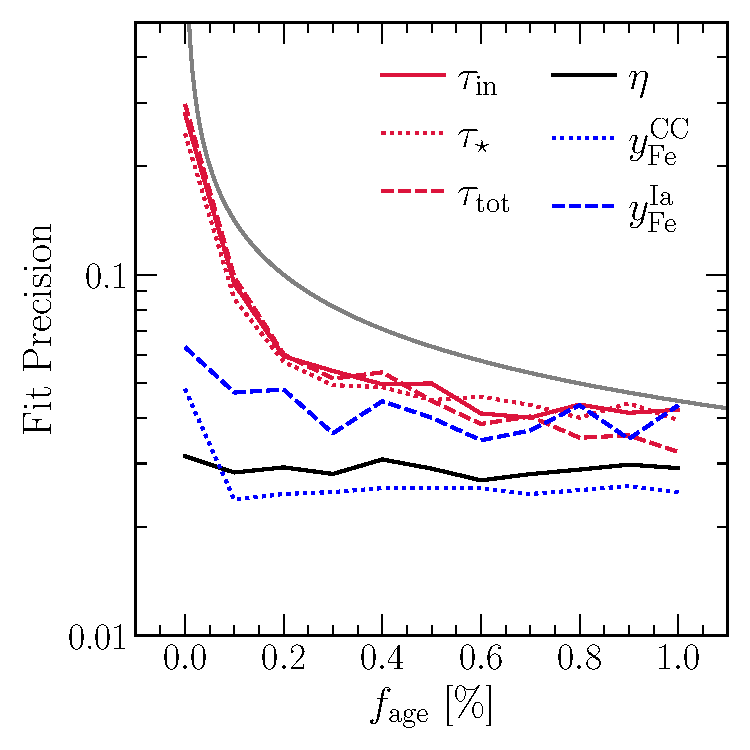
\includegraphics[scale = 0.55]{precision_agefrac.pdf}
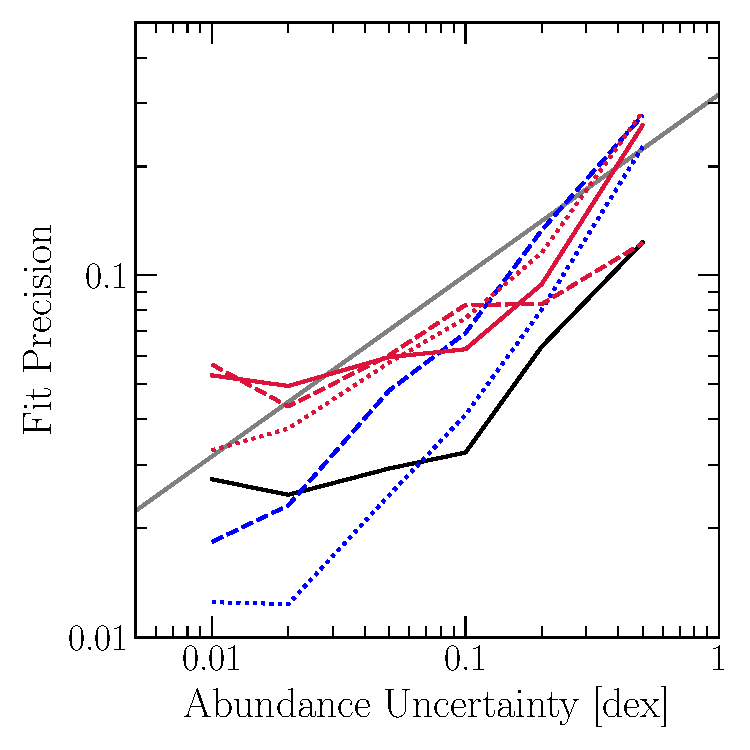
\includegraphics[scale = 0.55]{precision_abundanceuncertainty.pdf}
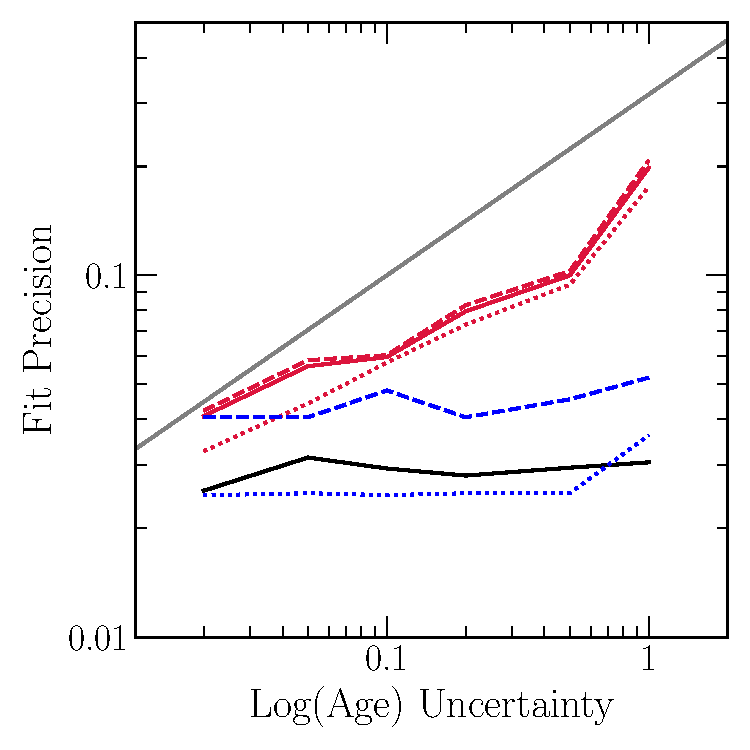
\includegraphics[scale = 0.55]{precision_ageuncertainty.pdf}
\caption{
Precision of our fitting method.
For a fit uncertainty~$\sigma$ and deviation from the known value
$\Delta\theta$, we compute precision according to
$\left|\Delta\theta\right| / \sigma$ for each of the six free parameters
in Table~\ref{dga:tab:recovered_values} and plot them as a function
of sample size (top left), the fraction of the sample with age information (top
right), abundance uncertainties (bottom left), and age uncertainties (bottom
right).
Grey lines in each panel denote~$x^{\pm0.5}$ scaling where~$x$ is the quantity
on the~$y$-axis.
We plot timescales in red, Fe yields in blue, and the mass-loading
factor~$\eta$ in black in all panels according to the legend.
}
\label{dga:fig:precision}
\end{figure*}

We have explored alternate parametrizations of our mock sample's evolutionary
history and indeed found that our method accurately recovers the parameters
in all cases.
For example, one is a case in which we build in a significant starburst,
finding that we accurately recover both the timing and the strength of the
burst.
We have also explored an infall rate that varies sinusoidally about some mean
value, mimicking natural fluctuations in the accretion history or a series of
minor starbursts.
Although idealized and potentially unrealistic, our likelihood function
accurately recovers the amplitude, phase and frequency in this case as well.
Of course, the parametrization itself must allow for such possibilities, but
we stick to smooth SFHs for the remainder of these tests.
\par
Fig.~\ref{dga:fig:precision} demonstrates how the uncertainty of each best-fit
parameter is affected by these details of the sample.
With differences in the normalization, the precision of each inferred parameter
scales with sample size approximately as~$N^{-0.5}$.
In general, the mass-loading factor~$\eta$ and the Fe yields are constrained
more precisely than the timescales.
The primary exception to this rule is when the abundance uncertainties are
large compared to the age uncertainties, in which case the Fe yields are
constrained to a similar precision as~$\tau_\text{in}$ and~$\tau_\star$
but~$\tau_\text{tot}$ is determined more precisely.
The Fe yields are, unsurprisingly, the most sensitive parameters to the
abundance uncertainties, while~$\eta$ can be determined with~$\sim$10\% precision
even with highly imprecise measurements ($\sigma_\text{[X/Y])} \approx 0.5$).
Even with imprecise abundances, the centroid of the MDF can still be robustly
determined with a sufficiently large sample, which allows a precise inference
of the strength of winds due to its impact on the equilibrium metallicity (for
an assumed scale of nucleosynthetic yields such as~$\yacc = 0.01$ in this
paper).
\par
Only the inferred timescales are impacted by the availability of age
information and the uncertainties thereof.
Even with order of magnitude uncertainties in stellar ages, however, the
evolutionary timescales of our mock samples are recovered to~$\sim$20\%
precision.
Interestingly the introduction of age information to the sample impacts the
fit uncertainty only for~$f_\text{age} \lesssim 30$\%.
Above this value, there is only marginal gain in the precision of best-fit
timescales.
These results suggest that authors seeking to determine best-fit evolutionary
parameters for one-zone models applied to any sample should focus their efforts
on sample size and precise abundance measurements with age information being
a secondary consideration.
Thankfully, abundances are generally easier than ages to measure on a
star-by-star basis~\citep{Soderblom2010, Chaplin2013}.

